%
% 4-geometrie.tex
%
% (c) 2022 Prof Dr Andreas Müller
%
\section{Weitere Geometrien
\label{buch:pde:section:geometrie}}
\kopfrechts{Weitere Geometrien}
Die Separationsmethode ist sehr erfolgreich.
Sie kann für beliebige Gebiete angwendet werden, wenn sie durch
Koordinatenlinien eines geeigneten Koordinatensystems begrenzt sind,
wie die Rechtecke in Abschnitt~\ref{buch:pde:section:rechteck}.
Ein Kreis oder Kreisring ist in Polarkoordinaten durch Kreise
um den Nullpunkt begrenzt, also durch eine Koordinatenlinie, auf
der die $\varrho$-Koordinate konstant ist und nur die Azimuth-Koordinaten
$\varphi$ variert.
Dies wird zum Beispiel im Kapitel~\ref{chapter:kreismembran}
durchgeführt.

Um eine der für die Physik zentralen partiellen Differentialgleichungen
wie
\begin{center}
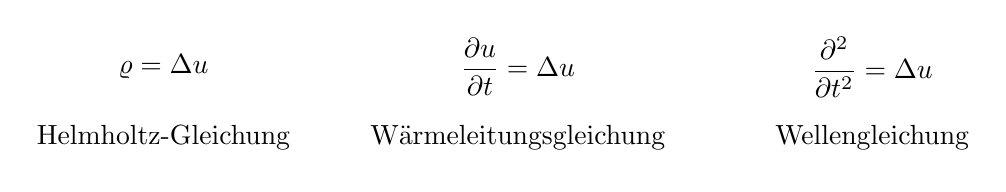
\begin{tikzpicture}[>=latex]
\def\l{0.9}
\begin{scope}[xshift=-4.5cm]
\node at (0,\l) {\(\displaystyle
\varrho = \Delta u
\mathstrut \)};
\node at (0,0) {Helmholtz-Gleichung\strut};
\end{scope}

\begin{scope}
\node at (0,\l) {\(\displaystyle
\frac{\partial u}{\partial t} = \Delta u
\mathstrut \)};
\node at (0,0) {Wärmeleitungsgleichung\strut};
\end{scope}

\begin{scope}[xshift=4.5cm]
\node at (0,\l) {\(\displaystyle
\frac{\partial^2}{\partial t^2} = \Delta u
\mathstrut \)};
\node at (0,0) {Wellengleichung\strut};
\end{scope}

\end{tikzpicture}
\end{center}
lösen zu können, muss auch der Laplace-Operator $\Delta$ in diesen
Koordinaten ausgedrückt werden.
Es ist zwar oft mühsam, eine solche Darstellung zu finden, aber
für die bekannten Koordinatensystem kann man sie auch in einschlägigen
Nachschlagewerken finden.

In Kapitel~\ref{chapter:parzyl} wird die Separationsmethode 
in parabolischen Koordinaten durchgeführt und führt auf die parabolischen
Zylinderfunktionen.
Und Kapitel~\ref{chapter:kugel} zeigt, wie dies auf einer Kugeloberfläche
in Kugelkoordinaten funktioniert.
Zusammen mit den Laguerre-Polynomen, die in Kapitel~\ref{chapter:laguerre}
eingeführt werden, entsteht eine Menge von Eigenfunktionen des
Laplace-Operators in Kugelkoordinaten.
Mit Kugelfunktionen wurden viele bedeutende Probleme gelöst.
Mit eines der wichtigsten dürfte die Lösung der Schrödingergleichung
für das Wasserstoff-Atom sein, welches zu einer Erklärung der
Gesetze von Balmer über die Wellenlängen der Wasserstoff-Spektrallinien
geführt hat.

Diese Beispiele illustrieren auch, dass die Randbedingungen einen
ganz entscheidenden Einfluss auf die Lösungen einer partiellen
Differentialgleichung haben.

In diesem Kapitel nicht besprochen wurde die Transformationsmethode
für partielle Differentialgleichungen \cite[chapter 5]{buch:partdiff}.
Zu jedem Koordinatensystem und jeder Lösung mit der Separationsmethode
gibt es auch eine passende Art von Integraltransformation, welche zur
Lösung des Problems mit der Transformationsmethode verwendet werden
kann ist.
Diese Idee wird in Kapitel~\ref{chapter:kreismembran}
am Beispiel der Hankeltransformation ausgeführt.




